%%%%%%%%%%%%%%%%%%%%%%%%%%%%%%%%%%%%%%%%%%%%%%%%%%%%%%%%%%%%%%%%%%%%%%%%%%%%%%%
%                         File: osa-revtex4-1.tex                             %
%                        Date: April 15, 2013                                 %
%                                                                             %
%                              BETA VERSION!                                  %
%                   JOSA A, JOSA B, Applied Optics, Optics Letters            %
%                                                                             %
%            This file requires the substyle file osajnl4-1.rtx,              %
%                   running under REVTeX 4.1 and LaTeX 2e                     %
%                                                                             %
%                   USE THE FOLLOWING REVTeX 4-1 OPTIONS:                     %
% \documentclass[osajnl,twocolumn,showpacs,superscriptaddress,10pt]{revtex4-1}%
%                    %% Use 11pt for Applied Optics                           %
%                                                                             %
%               (c) 2013 The Optical Society of America                       %
%                                                                             %
%%%%%%%%%%%%%%%%%%%%%%%%%%%%%%%%%%%%%%%%%%%%%%%%%%%%%%%%%%%%%%%%%%%%%%%%%%%%%%%

\documentclass[osajnl,twocolumn,showpacs,superscriptaddress,10pt]{revtex4-1} %% use 10pt for Applied Optics
%%\documentclass[osajnl,preprint,showpacs,superscriptaddress,12pt]{revtex4-1} %% use 12pt for preprint option
\usepackage{amsmath,amssymb,graphicx,float,enumerate}
\usepackage[cache=false]{minted}
\usepackage[utf8]{inputenc}
\graphicspath{ {../images/} }

\usepackage[colorlinks = true,
            linkcolor = black,
            urlcolor  = blue,
            citecolor = black,
            anchorcolor = blue]{hyperref}

\usepackage{silence}
\WarningFilter{revtex4-1}{Repair the float}

\begin{document}

\title{Redes y Comunicaciones}

\author{Ulises Jeremias Cornejo Fandos}
\affiliation{13566/7, Licenciatura en Informatica, Facultad de Informatica, UNLP}

\author{Federico Ramón Gasquez}
\affiliation{13598/6, Licenciatura en Informatica, Facultad de Informatica, UNLP}

\author{Lihuel Pablo Amoroso}
\affiliation{13497/2, Analista Programador Universitario, Facultad de Informatica, UNLP}

%%\begin{abstract}
%%\end{abstract}

\maketitle %% required

\onecolumngrid

\section{Introducción}

\textit{En la máquina virtual, instale el paquete radvd (sudo apt update; sudo apt install -y radvd).} \\

Utilizando la topología enlace-Ipv6.imn:

\begin{itemize}
    \item Analice las direcciones IPv6 de PC-A y PC-B:
    
    \begin{itemize}
        \item ¿Cuántas direcciones IP tiene cada interfaz?
        \item ¿Cuáles son?
        \item ¿Qué alcance tiene cada una de ellas?
    \end{itemize}
\end{itemize}

Analizando este aspecto de la topología observamos que ninguna de las interfaces
dispone de una IP asignada a simple vista. Sin embargo, luego de iniciar la topología,
se ejecuta el comando \textit{ifconfig} sobre cada uno de los hosts
viendo así las IPs asignadas a cada uno. En ambos casos se observan dos IPs asignadas, una de alcance local al enlace y otra de alcance global. \\

Es importante tener en cuenta que la IPv6 de alcance de Link Local no debe ser única a nivel Global,
sino solo en la red donde está contenida, y la misma comenzará en general con \textbf{ff80},
estando en el rango \textit{[fe80, febf]}. \\

Concretamente las IPs asignadas, con su correspondiente alcance, son:

\begin{itemize}
    \item \textbf{PC-A}
    
    \begin{itemize}
        \item inet6 addr: \textbf{fe80::200:ff:feaa:1/64} Scope: \textbf{Link}
        \item inet6 addr: \textbf{2001::200:ff:feaa:1/64} Scope: \textbf{Global}
    \end{itemize}

    \item \textbf{PC-B}
    
    \begin{itemize}
        \item inet6 addr: \textbf{fe80::200:ff:feaa:0/64} Scope: \textbf{Link}
        \item inet6 addr: \textbf{2001::200:ff:feaa:0/64} Scope: \textbf{Global}
    \end{itemize}
\end{itemize}

\section{Router advertisement - Análisis}

En PC-A, desconecte y conecte la interfaz mientras captura tráfico. \\

Analice los mensajes “Router Solicitation” y “Router advertisement”. \\

En la figura (\ref{image:router-solicitation-advertisement}) se observa la captura de paquetes durante 
la conexión de la interfaz eth0 en PC-A. \\

Los mensajes \textit{Router Advertisement} y \textit{Router Solicitationes} permiten que un nodo en un enlace descubra los routers 
en el mismo enlace. Cada interfaz de enrutador configurada en un enlace envía un mensaje de Router Advertisement, 
que tiene un valor de 134 en el campo \textit{Type} del encabezado del paquete ICMP, periódicamente a la dirección 
de multicast local de enlace de todos los nodos (\textit{FF02::1}). \\

Una interfaz de enrutador configurada también puede enviar un mensaje de Router Advertisement en respuesta a un mensaje 
de Router Solicitation desde un nodo en el mismo enlace. Este mensaje se envía a la dirección IPv6 de unicast del nodo 
que envió el mensaje de Router Solicitation.

Al iniciar el sistema, un host en un enlace envía un mensaje de Router Solicitation a la dirección de multicast de todos 
los routers (\textit{FF01}). El envío de un mensaje de Router Solicitation, que tiene un valor de 133 en el 
campo \textit{Type} del encabezado del paquete ICMP, permite al host configurar automáticamente su dirección IPv6 
inmediatamente en lugar de esperar el próximo mensaje periódico de anuncio del enrutador. \\

Debido a que un host en el inicio del sistema generalmente no tiene una dirección IPv6 de unicast, la dirección de origen 
en el mensaje de solicitud del enrutador suele ser la dirección IPv6 no especificada (0:0:0:0:0:0:0:0). 
Si el host tiene una dirección IPv6 de unicast, la dirección de origen es la dirección IPv6 de unicast 
de la interfaz del host que envía el mensaje de Router Solicitation. \\

\begin{figure}[H]
    \centering
    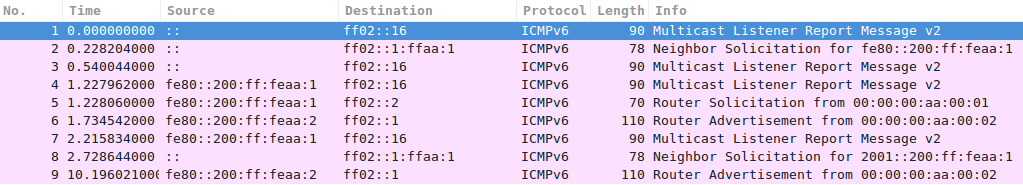
\includegraphics[width=0.95\textwidth]{router-solicitation-advertisement.png}
    \caption{Captura de paquetes durante la conexión de la interfaz eth0 en PC-A.}
    \label{image:router-solicitation-advertisement}
\end{figure}

\subsection{Router solicitation} 

\begin{itemize}
    \item ¿Cuál es el tipo y el código del mensaje?
    
    El mensaje es de tipo Router Solicitation con código 133.

    \item ¿Cuál es la MAC origen y la MAC destino?
    
    \begin{itemize}
        \item ¿Qué tipo de MAC es la MAC destino?
    \end{itemize}

    Se puede observar en la figura (\ref{image:router-solicitation-details}) que la MAC origen es 00:00:00:aa:00:01 y el valor del header \textit{Dst.} de Ethernet
    es \textbf{IPv6mcast\_02 (33:33:00:00:00:02)}. A partir de la definición provista en (\ref{superuser-ref}) se determina que
    las MAC destino son todas las direcciones asociadas a los routers de la red que, al ser en este caso único, es 00:00:00:aa:00:02.
    
    En la \href{https://tools.ietf.org/html/rfc2464#section-7}{RFC 2464} se puede notar como obtener la MAC de una interfaz
    específica a partir de un IPv6 multicast.
    
    \textit{Ethernet has "multicast" MAC addresses as well – any MAC address with the "group" bit set is technically a multicast address; IPv6 uses the prefix 33:33:*, while IPv4 uses 01:00:5e:*.}
    \label{superuser-ref}

    \item ¿Cuál es la IP origen y la IP destino?
    
    \begin{itemize}
        \item ¿Qué tipo de dirección es la IP origen y qué tipo de dirección es la IP destino?
    \end{itemize}

    La IP origen es \textit{fe80::200:ff:feaa:1} de tipo \textit{Link-local unicast} y la IP destino es \textit{ff02::02} de tipo \textit{Multicast}.

    \item ¿Qué datos puede destacar del mensaje ICMP?
    
    Como se menciona en el ejercicio anterior, se puede destacar que, cuando la interfaz perteneciente a uno de los nodos de la red, es desactivada y reactivada, el mismo genera un Router Solicitation, pidiéndole a todos los routers que se anuncien, es decir, Router Advertisement.
\end{itemize}

\begin{figure}[H]
    \centering
    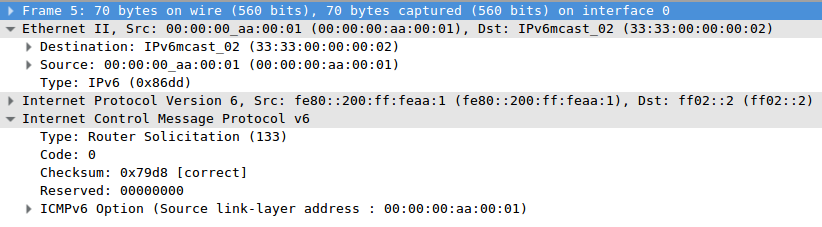
\includegraphics[width=0.95\textwidth]{router-solicitation-details.png}
    \caption{Información detallada del paquete 5 de la captura mostrada en la figura \ref{image:router-solicitation-advertisement}.}
    \label{image:router-solicitation-details}
\end{figure}

\subsection{Router advertisement}

\begin{itemize}
    \item ¿Cuál es el tipo y el código del mensaje?
    
    El mensaje es de tipo Router Advertisement con código 134.

    \item ¿Cuál es la MAC origen y la MAC destino?
    
    \begin{itemize}
        \item ¿Qué tipo de MAC es la MAC destino?
    \end{itemize}

    Se puede observar en la figura (\ref{image:router-advertisement-details}) que la MAC origen es 00:00:00:aa:00:02 y el valor del header \textit{Dst.} de Ethernet
    es \textbf{IPv6mcast\_01 (33:33:00:00:00:01)}. A partir de la definición provista en (\ref{superuser-ref}) se determina que
    las MAC destino es 00:00:00:aa:00:01.
    
    \item ¿Cuál es la IP origen y la IP destino?
    
    \begin{itemize}
        \item ¿Qué tipo de dirección es la IP origen y qué tipo de dirección es la IP destino?
    \end{itemize}
    
    La IP origen es \textit{ff02::02} de tipo \textit{Multicast} y la IP destino es \textit{fe80::200:ff:feaa:1} de tipo \textit{Link-local unicast}.

    \item ¿Qué datos puede destacar del mensaje ICMP? ¿Cuál es prefijo que se anuncia?
    
    Este mensaje surge como respuesta a un Router Solicitation o para mantener a los nodos informados. El prefijo
    que se sugiere es el \textit{2001::} correspondiente a \textbf{Global unicast} de IPv6.
\end{itemize}

\begin{figure}[H]
    \centering
    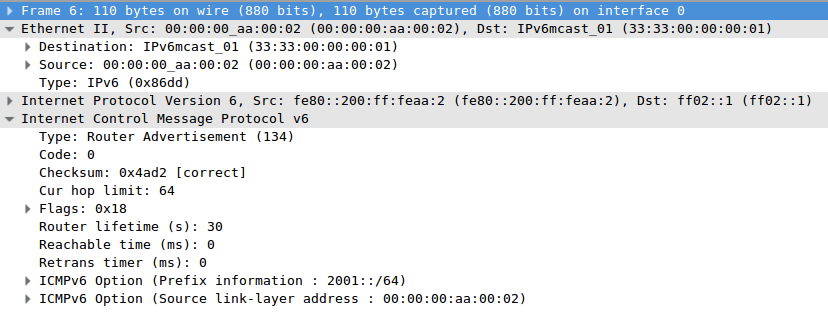
\includegraphics[width=0.95\textwidth]{router-advertisement-details.png}
    \caption{Información detallada del paquete 6 de la captura mostrada en la figura \ref{image:router-solicitation-advertisement}.}
    \label{image:router-advertisement-details}
\end{figure}

\section{Análisis de rutas}

Visualice la tabla de rutas de IPv6:

\begin{itemize}
    \item ¿Cuál es el default GW de PC-A? ¿Qué alcance tiene dicha dirección?
\end{itemize}

\textit{Verifique conectividad entre PC-A y “SERVER”.} \\

Para visualizar la tabla de rutas de IPv6, se ejecuta el comando \textbf{ip -6 route}, \textit{ó ip -6 route list} obteniendo
una tabla como la que se observa en la figura (\ref{image:ip-route}). \\

En la misma se puede observar que el default gateway de PC-A es \textbf{fe80:200:ff:feaa:2}, una IPv6 de alcance de Link local.

\begin{figure}[H]
    \centering
    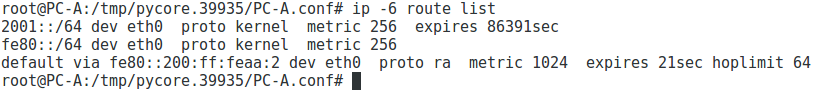
\includegraphics[width=0.95\textwidth]{ip-route.png}
    \caption{Tabla de rutas de IPv6.}
    \label{image:ip-route}
\end{figure}

Luego se hace un ping desde PC-A a la IPv6 Global de SERVER para verificar la conectividad, como
se ve en la figura (\ref{image:ping-pca-server}). En la figura (\ref{tcpdump-server}) se observa la captura de tráfico
en SERVER.

\begin{figure}[H]
    \centering
    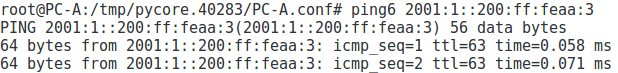
\includegraphics[width=0.95\textwidth]{ping-pca-server.png}
    \caption{Ping desde PC-A a SERVER.}
    \label{image:ping-pca-server}
\end{figure}

\begin{figure}[H]
    \centering
    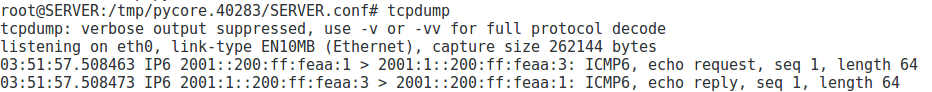
\includegraphics[width=0.95\textwidth]{tcpdump-server.png}
    \caption{Captura de tráfico en SERVER utilizando tcpdump.}
    \label{image:tcpdump-server}
\end{figure}

\section{Neighbor discovery - Análisis}

\textit{Desde PC-A haga un ping a la IPv6 global de PC-B mientras captura tráfico ICMPv6 en
PC-B. Analice los mensajes “Neighbor Solicitation” y “Neighbor Advertisement”.} \\

Primero se obtiene la IPv6 global de PC-B utilizando el comando \textit{ifconfig} obteniendo
la siguiente IP, \textbf{2001::200:ff:feaa:0}. \\

Desde PC-A se ejecuta el comando \textbf{ping6} para hacer un ping a la IPv6 de PC-B
mientras se capturan el tráfico ICMPv6 en PC-B. \\

\begin{figure}[H]
    \centering
    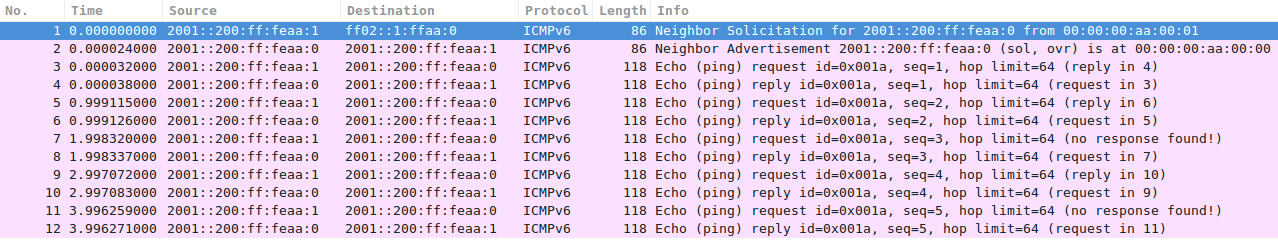
\includegraphics[width=0.95\textwidth]{neighbor-solicitation-advertisement.png}
    \caption{Captura de paquetes del ping de PC-A a IPv6 global de PC-B.}
    \label{image:neighbor-solicitation-advertisement}
\end{figure}

\subsection{Neighbor solicitation}

\begin{itemize}
    \item ¿Cuál es el tipo y el código del mensaje?
    
    Es un código de tipo Neighbor Solicitation de código 135.

    \item ¿Cuál es la MAC origen y la MAC destino?
    
    \begin{itemize}
        \item ¿Qué tipo de MAC es la MAC destino?
    \end{itemize}

    Se puede observar en la figura (\ref{image:image:neighbor-solicitation-details}) que la MAC origen es 00:00:00:aa:00:01 de tipo Unicast y el valor del header \textit{Dst.} de Ethernet
    es \textbf{IPv6mcast\_ff:aa:00:00 (33:33:ff:aa:00:00)} de tipo Multicast ya que tiene asociada la IPv6 ff02::1:ffaa:0. Se determina que la MAC destino efectiva es 00:00:00:aa:00:00 al ser un único router.
    
    \item ¿Cuál es la IP origen y la IP destino?
    
    \begin{itemize}
        \item ¿Qué tipo de IP es la IP destino?
    \end{itemize}

    La IP origen es \textit{2001::200:ff:feaa:1} de tipo \textit{Global} y la IP destino es \textit{2001::200:ff:feaa:0} de tipo \textit{Global}.
    
    \item ¿Qué datos puede destacar del mensaje ICMP?
    
    El mensaje \textbf{Neighbor Solicitation} se utiliza determinar la dirección MAC de un nodo específico dentro de la red o para saber si éste sigue respondiendo a la dirección MAC que se encuentra almacenada en la caché.
\end{itemize}

\begin{figure}[H]
    \centering
    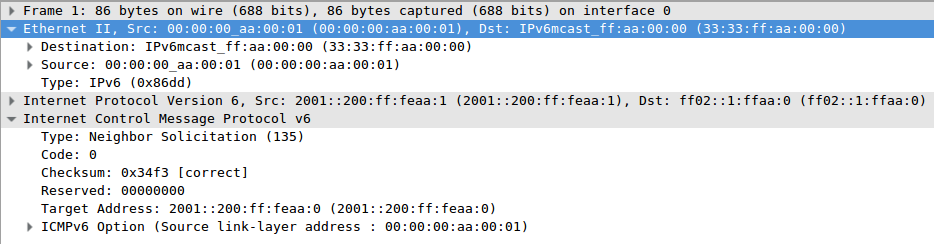
\includegraphics[width=0.95\textwidth]{neighbor-solicitation-details.png}
    \caption{Información detallada del paquete 1 de la captura mostrada en la figura \ref{image:neighbor-solicitation-advertisement}.}
    \label{image:neighbor-solicitation-details}
\end{figure}

\subsection{Neighbor Advertisement}

\begin{itemize}
    \item ¿Cuál es el tipo y el código del mensaje?
    
    Es un mensaje del tipo Neighbor Advertisement con código 136.

    \item ¿Cuál es la MAC origen y la MAC destino?
    
    
    \begin{itemize}
        \item ¿Qué tipo de MAC es la MAC destino?
    \end{itemize}

    La dirección MAC origen es 00:00:00:aa:00:00 y la destino es 00:00:00:aa:00:01.
    Al igual que en el caso del Neighbor Solicitation, la MAC es de tipo multicast.
    
    \item ¿Cuál es la IP origen y la IP destino?
    
    \begin{itemize}
        \item ¿Qué tipo de IP es la IP destino?
    \end{itemize}

    La dirección IPv6 origen es 2001::200:ff:feaa:0 y la IPv6 destino es la IP 2001::200:ff:feaa:1, ambas de tipo \textit{Global}.
    
    \item ¿Qué datos puede destacar del mensaje ICMP?

    Este mensaje se dispara automáticamente al recibir el mensaje anterior (neighbor solicitation) o se genera cuando se va a realizar un cambio en su dirección.
\end{itemize}

\begin{figure}[H]
    \centering
    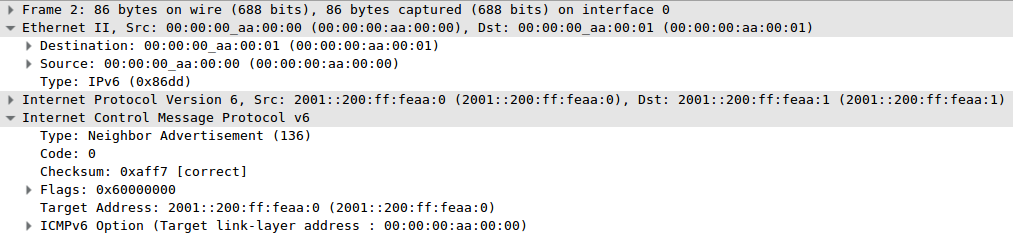
\includegraphics[width=0.95\textwidth]{neighbor-advertisement-details.png}
    \caption{Información detallada del paquete 2 de la captura mostrada en la figura \ref{image:neighbor-advertisement-advertisement}.}
    \label{image:neighbor-advertisement-details}
\end{figure}

\textit{\textbf{Visualice la tabla de caché de NDP de PC-A utilizando las herramientas provistas por
iproute2.}} \\

Podemos observar la tabla de caché de NDP de PC-A ejecutando el comando \textit{ip neighbor show} como se ve
en la figura (\ref{image:ndp-table}).

\begin{figure}[H]
    \centering
    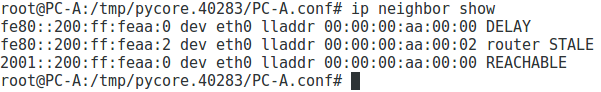
\includegraphics[width=0.95\textwidth]{ndp-table.png}
    \caption{Tabla de caché de NDP de PC-A.}
    \label{image:ndp-table}
\end{figure}

\end{document}
